\documentclass{article}
\usepackage[T1]{fontenc}
\usepackage[utf8]{inputenc}
\usepackage{amsmath,amsfonts,amssymb,amsopn,amscd,amsthm, mathrsfs}
\usepackage{xcolor}
\usepackage{tikz}
\usepackage{xcolor}
\usetikzlibrary{shapes.misc,arrows,decorations.pathmorphing,backgrounds,positioning,fit,petri,shapes,petri,cd,arrows.meta,patterns,fadings,calc}

\begin{document}

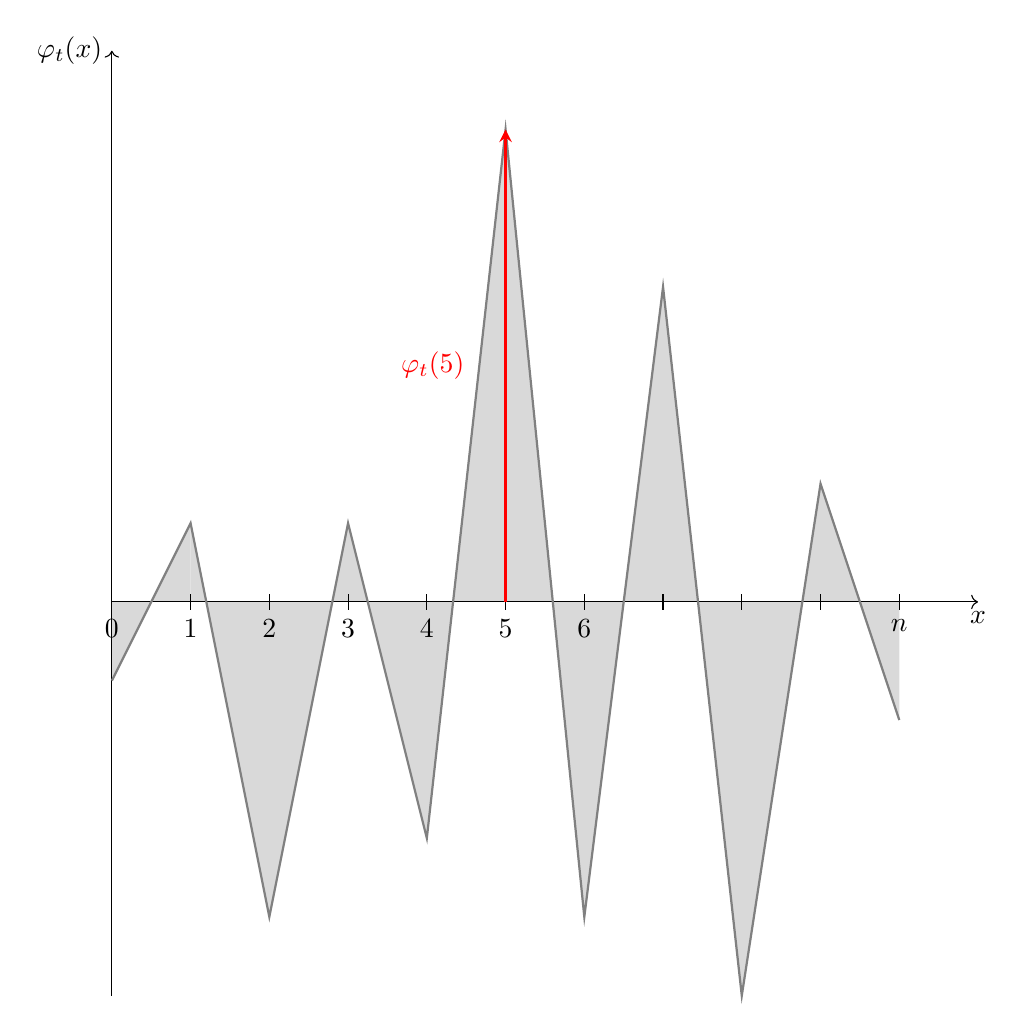
\begin{tikzpicture}[scale=1]
\fill[gray!30] (0,0) -- (0,-1) -- (0.5,0) -- cycle;
\fill[gray!30] (0.5,0) -- (1,1) -- (1,0) -- cycle;
\fill[gray!30] (1,0) -- (1,1) -- (6/5,0) -- cycle;
\fill[gray!30] (6/5,0) -- (2,-4) -- (14/5,0) -- cycle;
\fill[gray!30] (14/5,0) -- (3,1) -- (3.25,0) -- cycle;
\fill[gray!30] (3.25,0) -- (4,-3) -- (13/3,0) -- cycle;
\fill[gray!30] (13/3,0) -- (5,6) -- (5.6,0) -- cycle;
\fill[gray!30] (5.6,0) -- (6,-4) -- (6.5,0) -- cycle;
\fill[gray!30] (6.5,0) -- (7,4)-- (67/9,0) -- cycle;
\fill[gray!30] (67/9,0) -- (8,-5) -- (114/13,0) -- cycle;
\fill[gray!30] (114/13,0) -- (9,1.5) -- (9.5,0) -- cycle;
\fill[gray!30] (9.5,0) -- (10,-1.5) -- (10,0) -- cycle;
% Axes)
\draw[->] (0,-5) -- (0,7) node[left] {{$\varphi_t (x)$}};
\draw[->] (0,0) -- (11,0) node[below] {{$x$}};


% Graduations et numérotation sur l'axe x
\foreach \x in {0,1,2,3,4,5,6}{
    \draw (\x,0.1) -- (\x,-0.1) node[below] {{$\x$}};
 }
\foreach \x in {7,8,9}{
    \draw (\x,0.1) -- (\x,-0.1) node[below]{$$};}       
\draw  (10,0.1) -- (10,-0.1) node[below] {{$n$}};   

% Ligne brisée
\draw[gray, thick] (0,-1) -- (1,1) -- (2,-4) -- (3,1) -- (4,-3) -- (5,6) --(6,-4)-- (7,4) -- (8,-5) -- (9,1.5) -- (10,-1.5);




% Flèche rouge et légende
\draw[red, line width=1pt, >=stealth, ->] (5,0) -- (5,6);
\node[left] at (4.6,3) {\textcolor{red}{{$\varphi_t(5)$}}};
\end{tikzpicture}

\end{document}